\documentclass{article}
\usepackage[utf8]{inputenc}

\title{CS 376 : HW 4 - Continuous Systems}
\author{Fred Eisele }
\date{October 2014}

\usepackage{natbib}
\usepackage{graphicx}
\usepackage{tikz}
\usetikzlibrary{shapes,arrows}
\usepackage{amsfonts}

\begin{document}

\maketitle

This problem set is taken from \citep{IntroEmbedSys} chapter 2 : Problem 6.


This system makes use of a helicopter model Figure \ref{fig:helicopter_plant}.
In this model the value of $a = 5$ and $T_top = 4$.
This Simulink model corresponds to the mathematical model.
For the Scale we have \ldots

\begin{equation}
\forall t \in \mathbb{R} ,  \qquad
y_1(t) = a x_1(t), \qquad
a & = \frac{1}{I_{yy}} = 4 \quad \text{units}
\end{equation}

\ldots and for the Integrator \ldots
\begin{equation}
\forall t \in \mathbb{R},  \qquad
y_2(t) = i + \int_0^t x_2(\tau) \, \mathrm{d}\tau , \qquad
i = \dot{\theta}(0) = 0
\end{equation}

\begin{figure}[h!]
\centering
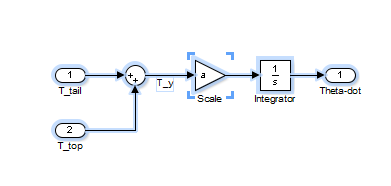
\includegraphics[scale=0.8]{helicopter_model.png}
\caption{the helicopter plant model (SimuLink)}
\label{fig:helicopter_plant}
\end{figure}

Using Simulink and its continuous-time modeling component
I have built a model of the helicopter control
system shown in Figure \ref{fig:control_system}.
This model has an upper section that models a system
with a proportional (P) controller and a lower section
that models a proportional-integrator (PI) controller.
The P-controller subsystem illustrates problem a)
with the lower subsystem modeling problem b).
These are placed together so that the inputs and outputs
may be shared.

\begin{figure}[h!]
\centering
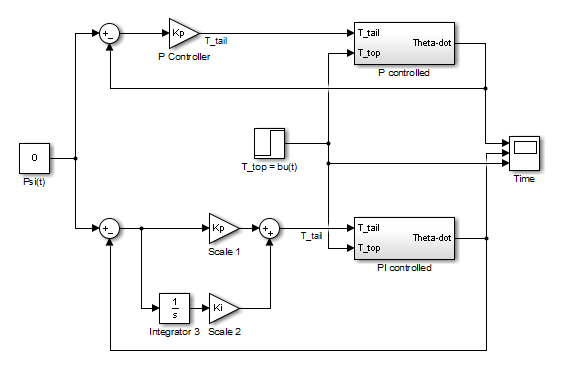
\includegraphics[scale=0.8]{controller_model.png}
\caption{the control systems models (SimuLink)}
\label{fig:control_system}
\end{figure}

\section{P-controller system}

Given some reasonable input parameters the
actual angular velocity, $\dot{\theta}$, is shown
as a function of time.
The initial and operating conditions
specify that the desired angular velocity
is zero, $\phi (t) = 0$, and that the
top-rotor torque is non-zero,
$T_{top}(t) = b u(t)$ moving to that
value as a step function.
Given are plots for several values of $K_p$.


Once the $T_{top}$ has changed a new stable but
typically non-zero $\dot{\theta}$ is approached asymtotically.
Larger values of $K_p$ cause the convergence
to happen more quickly and decrease the value of
the stable $\dot{\theta}$.


\section{PI-controller system}
The lower portion of Figure \ref{fig:control_system}
replaces the proportional (P) controller of the upper system
with a propotional-integrator (PI) controller.
This alternative controller has two parameter $K_p$ and $K_i$.
Experiment with the values of these parameters,
give some plots of the behavior with the
same inputs as in part (a), and discuss the
behavior of this controller in contrast
to the one of part (a).

Once the $T_{top}$ has changed a new (typically non-zero)
$\dot{\theta}$ is approached controlled-variable, $\Psi = 0$,
is approached asymtotically by $\dot{\theta}$
after $T_{top}$ changes.
Larger values of $K_p$ cause the convergence
to happen more quickly.

\begin{figure}[h!]
\centering
\includegraphics[scale=0.8]{theta_dot_kp_100_ki_12.png}
\caption{the control systems models (SimuLink)}
\label{fig:td_100_12}
\end{figure}


\begin{figure}[h!]
\centering
\includegraphics[scale=0.8]{theta_dot_kp_30_ki_12.png}
\caption{the control systems models (SimuLink)}
\label{fig:td_30_12}
\end{figure}

\begin{figure}[h!]
\centering
\includegraphics[scale=0.8]{theta_dot_kp_30_ki_120.png}
\caption{the control systems models (SimuLink)}
\label{fig:td_30_120}
\end{figure}

\begin{figure}[h!]
\centering
\includegraphics[scale=0.8]{theta_dot_kp_30_ki_12k.png}
\caption{the control systems models (SimuLink)}
\label{fig:td_30_1200}
\end{figure}

\begin{figure}[h!]
\centering
\includegraphics[scale=0.8]{theta_dot_kp_30_ki_24.png}
\caption{the control systems models (SimuLink)}
\label{fig:td_30_24}
\end{figure}

\begin{figure}[h!]
\centering
\includegraphics[scale=0.8]{theta_dot_kp_40_ki_12.png}
\caption{the control systems models (SimuLink)}
\label{fig:td_40_12}
\end{figure}

\bibliographystyle{plain}
\bibliography{references}
\end{document}
